% =====================================================================
% presentation.tex — Final project slides (Beamer, metropolis theme)
%
% Structure follows docs/university_deliverables/PRESENTATION.md
% (15 slides + Q&A backup appendix). Red [TODO ...] markers = fill
% after the Phase D retrain, then delete.
%
% Build:  pdflatex presentation.tex   (twice, for nav/refs)
% Figures resolve from docs/figures/ and checkpoints/samples/.
% =====================================================================
\documentclass[aspectratio=169,10pt]{beamer}

\usetheme{metropolis}
\usepackage{booktabs}
\usepackage{graphicx}
\usepackage{xcolor}

\graphicspath{{../../figures/}{../../../checkpoints/samples/}}

% --- Accent color (tweak to taste) ---
\definecolor{accent}{HTML}{EB5601}
\setbeamercolor{progress bar}{fg=accent}
\setbeamercolor{alerted text}{fg=accent}

% --- TODO marker: loud on purpose, delete before delivery ---
\newcommand{\todo}[1]{\textcolor{red}{\textbf{[TODO: #1]}}}

% --- Metadata ---
\title{Multi-Task Semantic-Geometric Fusion for\\Robotic Part Affordance Extraction}
\subtitle{Computer Vision --- Final Project}
\author{Francesco Dorati}
\date{June 2026}

\begin{document}

% =====================================================================
% 1. TITLE
% =====================================================================
\begin{frame}
  \titlepage
  % Hero image: mug with three simultaneous affordances
  \begin{center}
    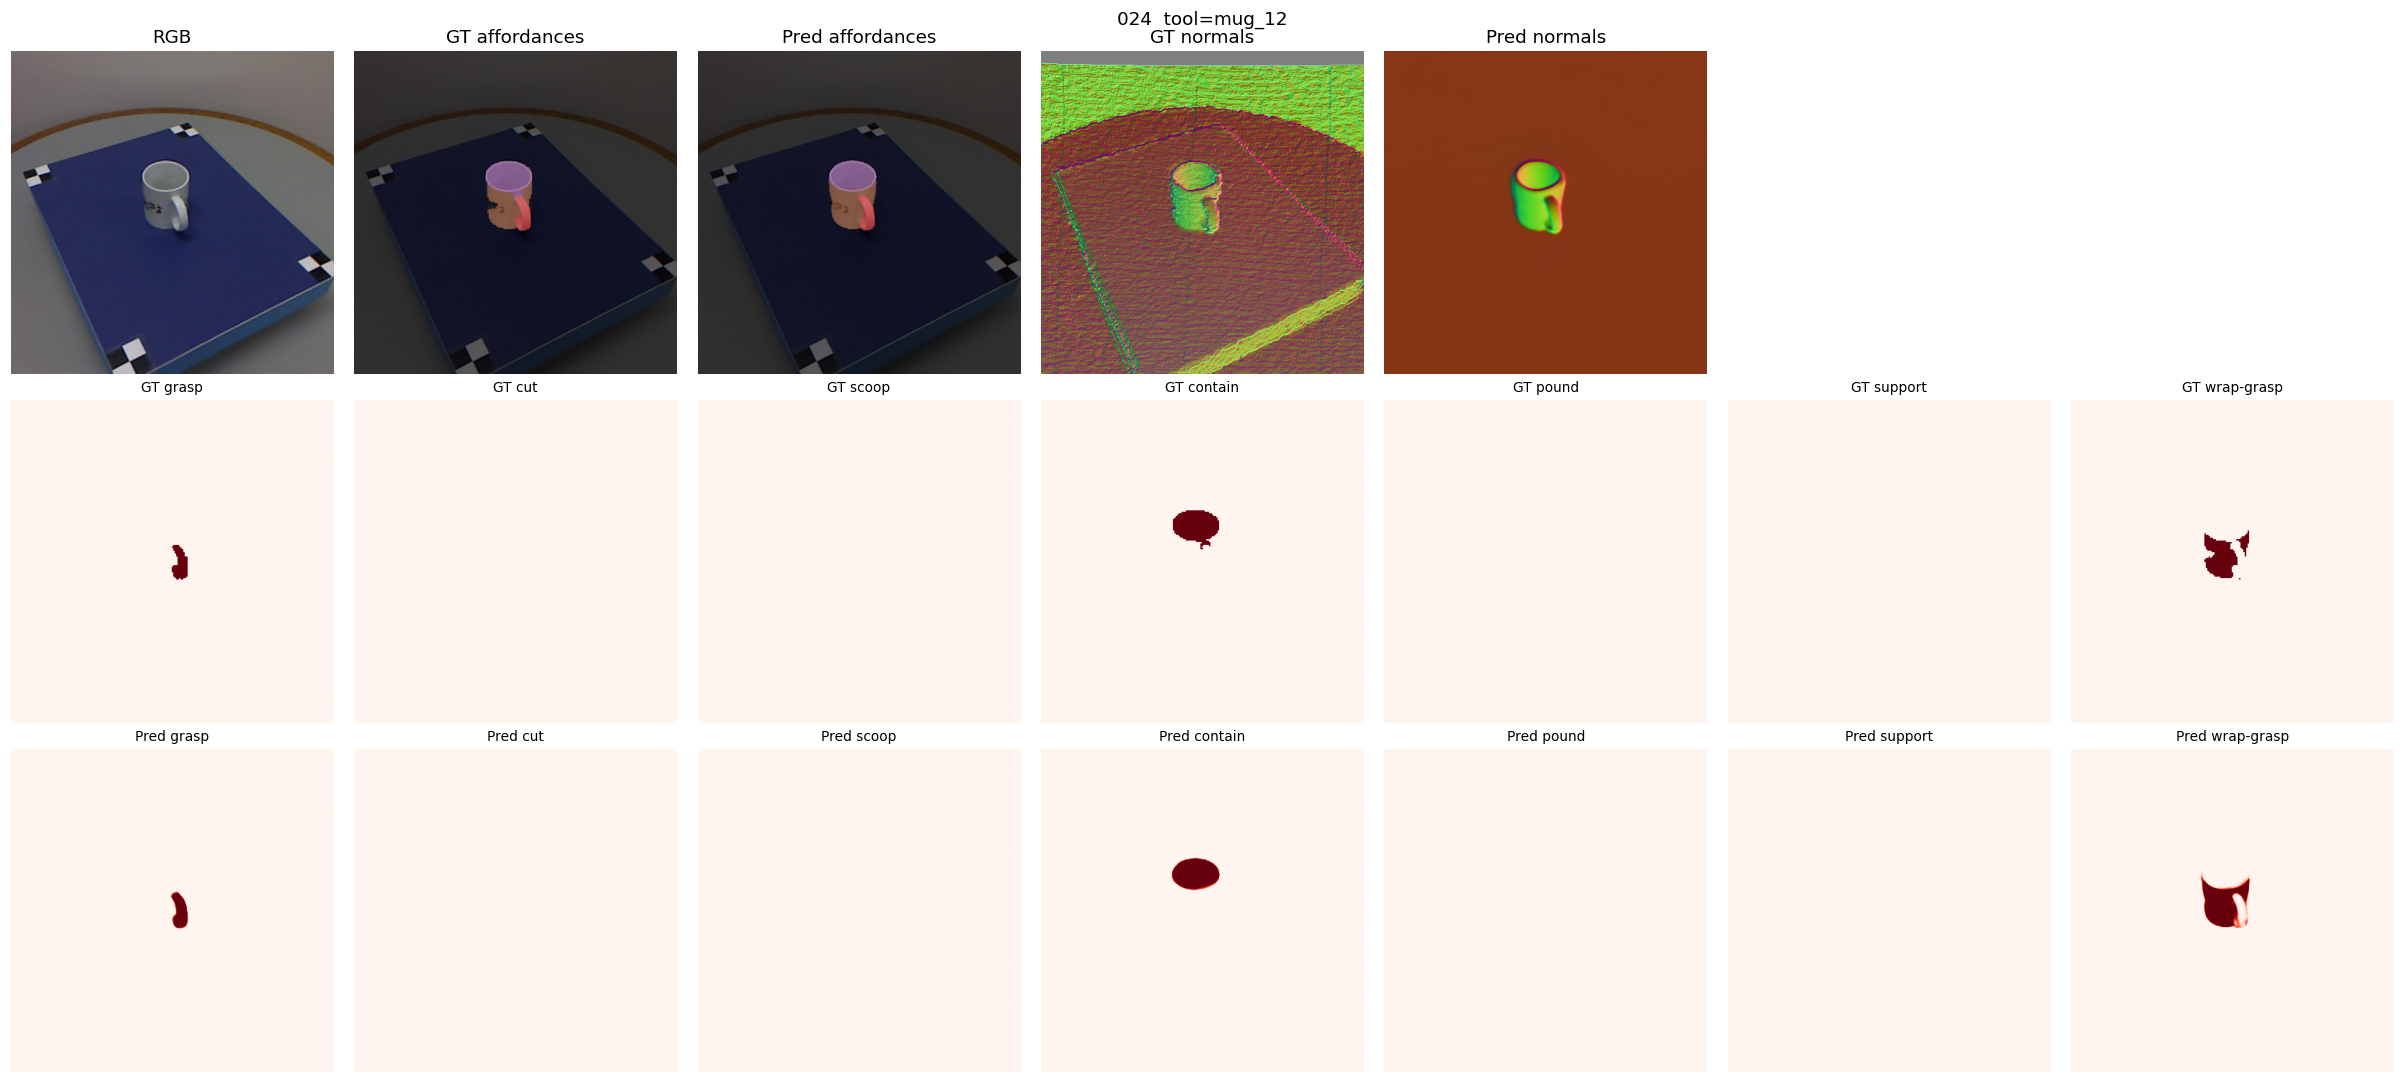
\includegraphics[height=0.35\textheight]{sample_mug.png}
  \end{center}
\end{frame}

% =====================================================================
% 2. THE PROBLEM
% =====================================================================
\begin{frame}{The problem: \emph{what} is not enough --- robots need \emph{how}}
  \begin{columns}[T]
    \begin{column}{0.55\textwidth}
      \begin{itemize}
        \item A robot sees a tool it has never encountered.
        \item Recognising ``this is a knife'' does not tell it
              \alert{where to grab} or \alert{how to approach}.
        \item \textbf{Affordance}: the functional role of each object
              \emph{region} --- the blade cuts, the handle is grasped.
      \end{itemize}
    \end{column}
    \begin{column}{0.42\textwidth}
      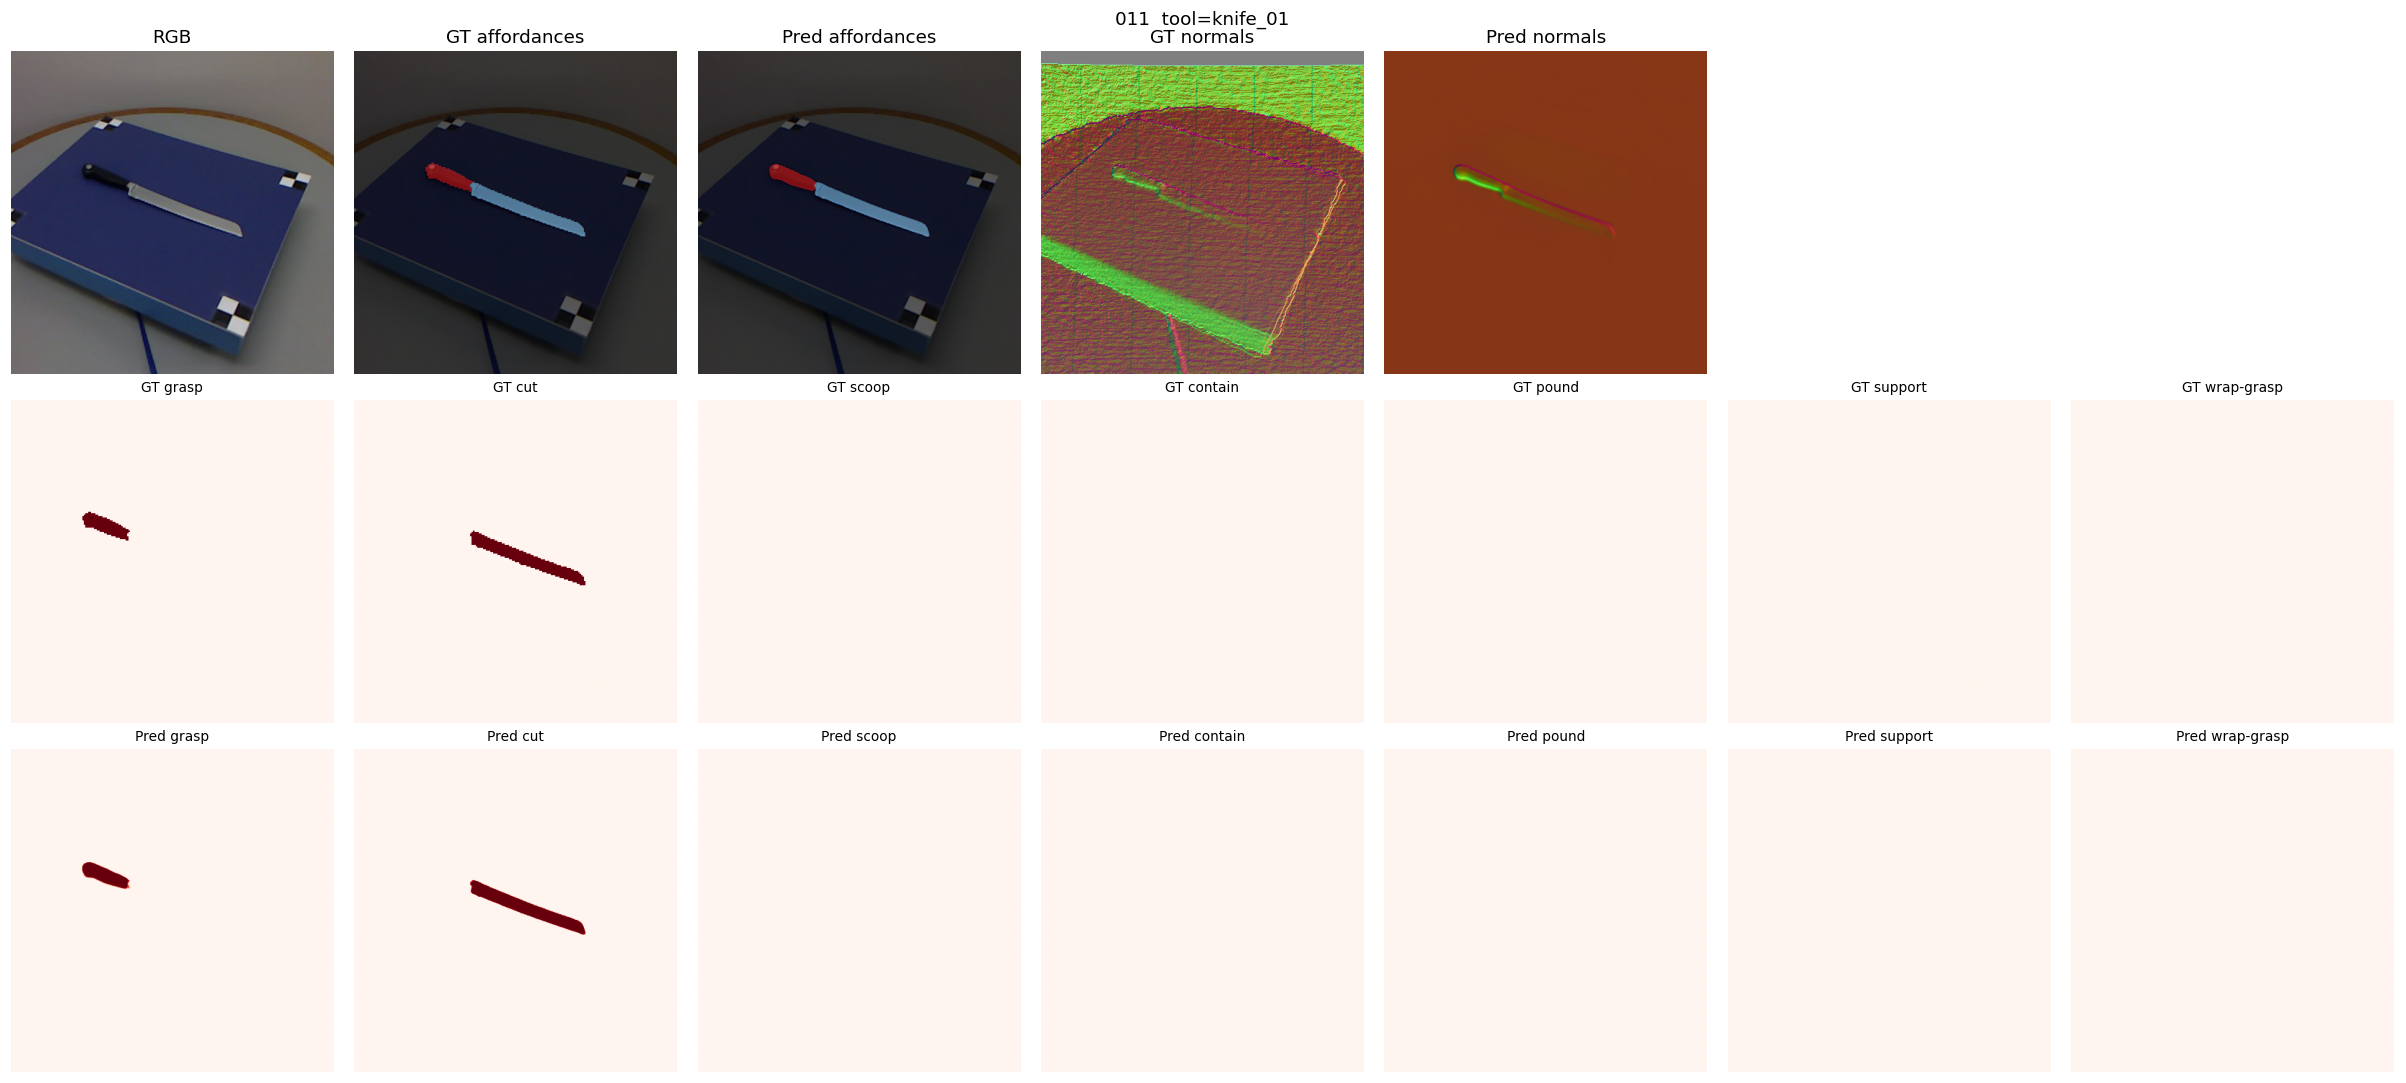
\includegraphics[width=\textwidth]{sample_knife_cut_grasp.png}
    \end{column}
  \end{columns}
\end{frame}

% =====================================================================
% 3. WHY THIS MATTERS
% =====================================================================
\begin{frame}{Why this matters: perception for humanoids}
  \begin{itemize}
    \item Humanoids in kitchens and workshops face \emph{open-world} objects:
          no CAD models, no guaranteed depth (fails on glass, reflective surfaces).
    \item Goal: an \alert{RGB-only perception primitive} producing a full
          grasp packet --- target region $(X, Y, Z)$ + approach vector
          $(N_x, N_y, N_z)$.
    \item Designed as the \emph{``where do I touch this?''} module of a
          manipulation stack: scene parser $\rightarrow$ \textbf{this model}
          $\rightarrow$ motion planner.
  \end{itemize}
  \medskip
  \begin{center}
    \small\itshape Built for a real robotics use case, not only a benchmark.
  \end{center}
\end{frame}

% =====================================================================
% 4. TASK & DATASET
% =====================================================================
\begin{frame}{Task and dataset}
  \begin{columns}[T]
    \begin{column}{0.55\textwidth}
      \textbf{Two joint outputs} from one RGB image:
      \begin{itemize}
        \item 7-channel \alert{multi-label} affordance mask
              (\texttt{grasp, cut, scoop, contain, pound, support, wrap-grasp})
        \item Dense \alert{surface normals} (unit vectors)
      \end{itemize}
      \medskip
      \textbf{UMD Part Affordance Dataset}
      \begin{itemize}
        \item $\sim$28K RGB-D turntable images, pixel-level labels
        \item \alert{Instance split}: val tools \emph{never} seen in training
              $\rightarrow$ measures cross-instance generalisation
      \end{itemize}
    \end{column}
    \begin{column}{0.42\textwidth}
      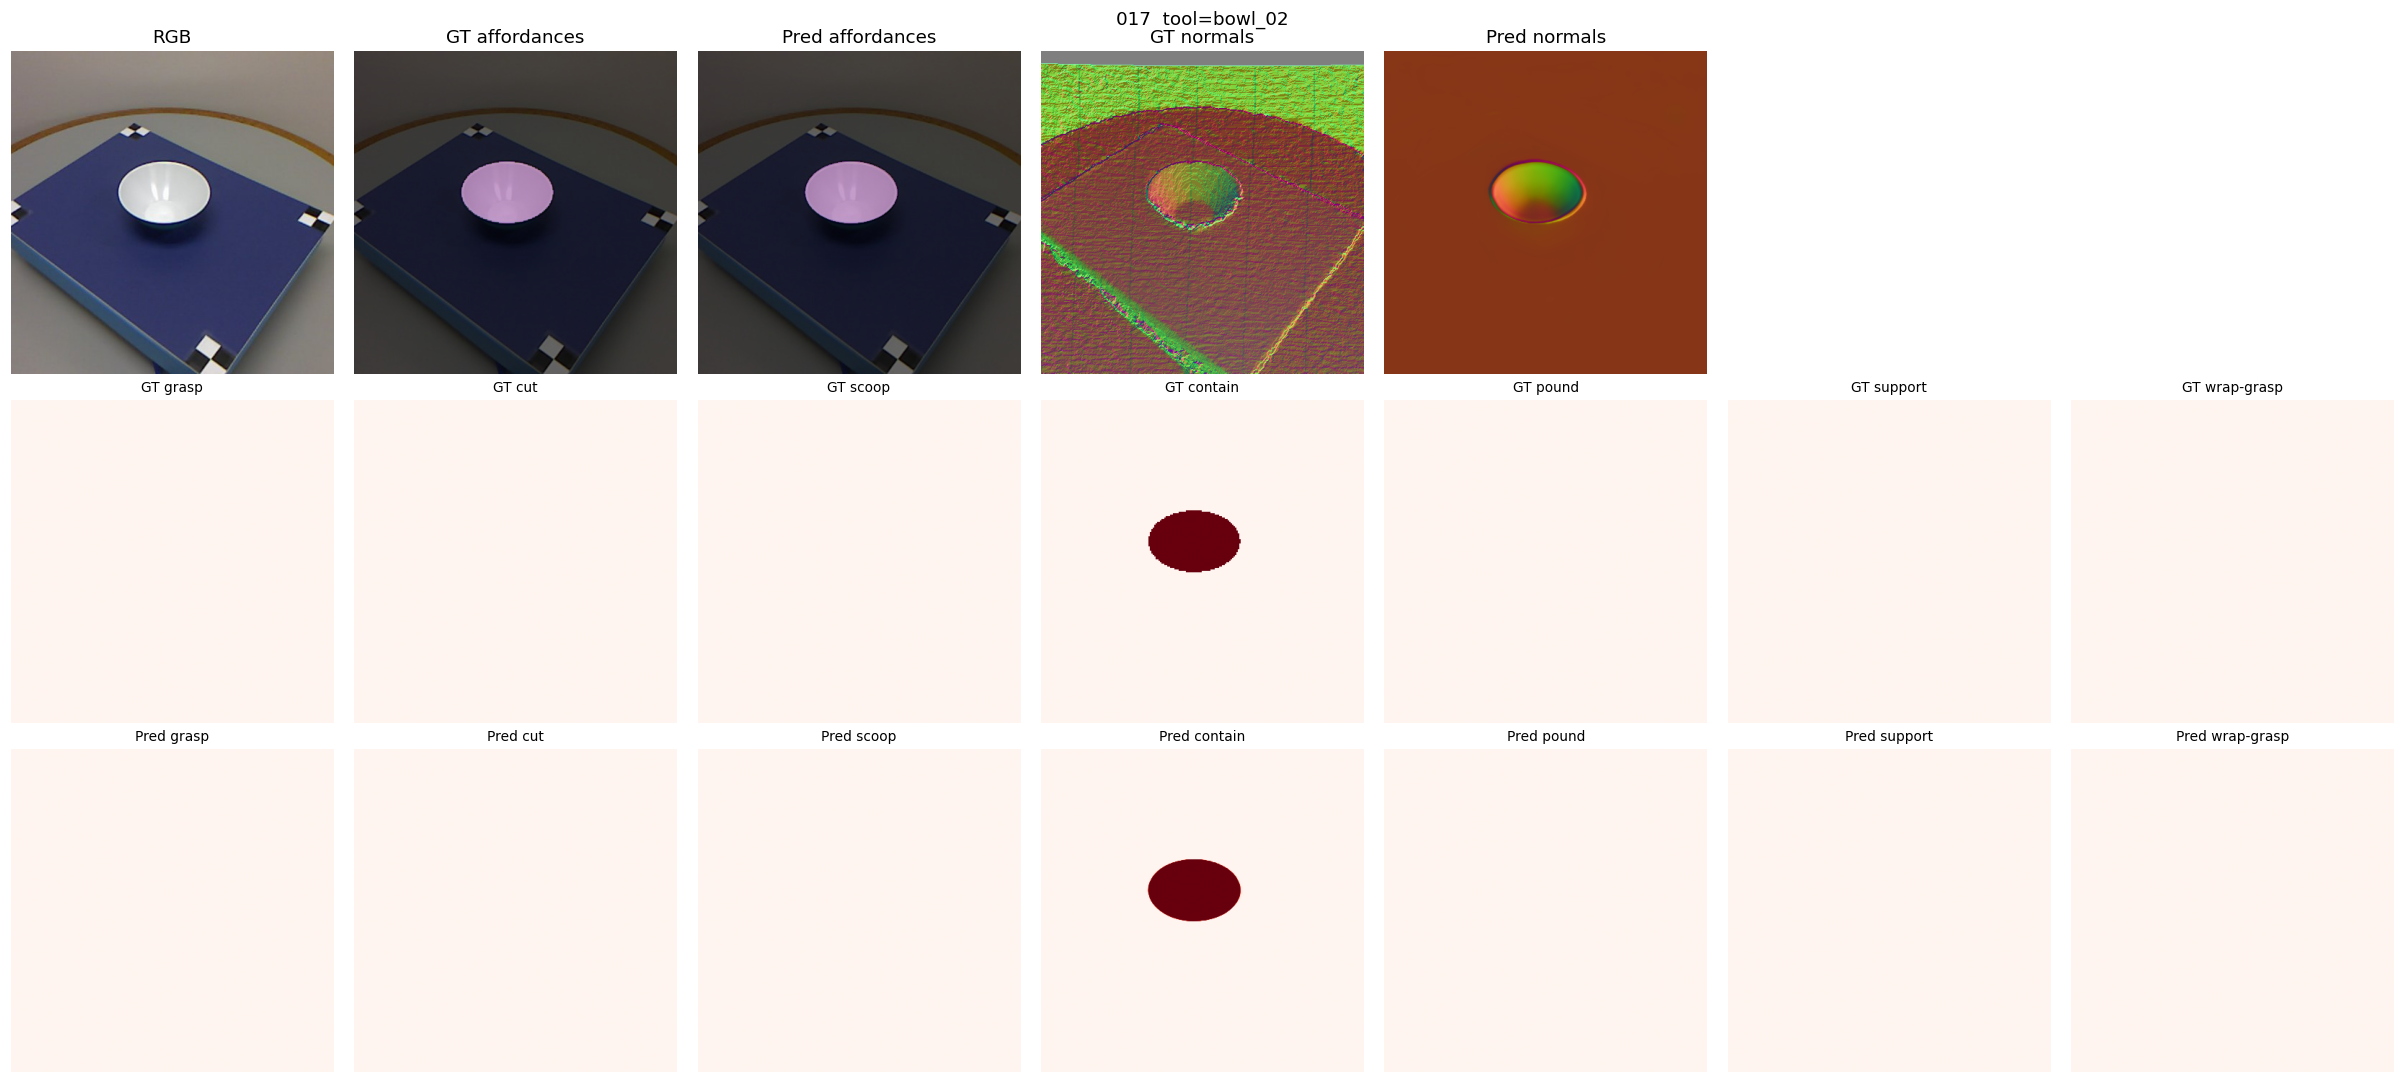
\includegraphics[width=\textwidth]{sample_bowl_contain.png}
      \par\smallskip
      {\scriptsize One GT sample: RGB / labels / normals}
    \end{column}
  \end{columns}
\end{frame}

% =====================================================================
% 5. ARCHITECTURE
% =====================================================================
\begin{frame}{Architecture: frozen foundation + lightweight trainable decoder}
  \begin{center}
    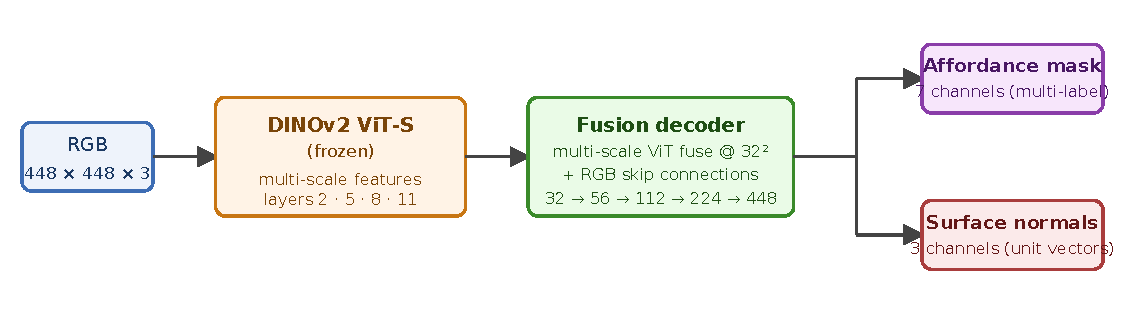
\includegraphics[width=0.78\textwidth]{architecture_overview.pdf}
  \end{center}
  \begin{itemize}\small
    \item \textbf{Frozen DINOv2 ViT-S}: 142M-image priors; fine-tuning on
          28K narrow images would destroy them.
    \item \textbf{Multi-scale taps} (layers 2/5/8/11, DPT-style): early layers
          keep spatial detail, late layers carry semantics.
    \item \textbf{RGB skip stem}: a $32{\times}32$ token grid cannot recover
          $448{\times}448$ edges --- the stem keeps them alive.
          Only \alert{3.6M trainable parameters}.
  \end{itemize}
\end{frame}

% =====================================================================
% 6. LOSSES
% =====================================================================
\begin{frame}{Training objective}
  \begin{equation*}
    \mathcal{L} \;=\; \mathcal{L}_{\text{mask}}
      \;+\; 5.0\cdot\mathcal{L}_{\text{normal}}
      \;+\; 0.5\cdot\mathcal{L}_{\text{smooth}}
  \end{equation*}
  \begin{itemize}
    \item \textbf{Mask}: per-channel BCE + soft Dice. Affordances cover
          $<1\%$ of pixels --- BCE alone collapses to ``all background''.
    \item \textbf{Normals}: masked cosine distance --- supervised only where
          the robot will actually touch.
    \item \textbf{Smoothness}: edge-aware --- normals stay smooth on flat
          surfaces, may break at image edges.
  \end{itemize}
  \medskip
  \textbf{Why multi-label, not softmax?} A trowel face is simultaneously
  \texttt{support} \emph{and} \texttt{scoop}; softmax would force a false
  exclusivity.
\end{frame}

% =====================================================================
% 7. STORY PART 1 — INVISIBLE BOWLS
% =====================================================================
\begin{frame}{The iterative story, part 1: the invisible bowls}
  \begin{columns}[T]
    \begin{column}{0.55\textwidth}
      \textbf{Phase A} --- binary baseline (\texttt{grasp}$\cup$\texttt{wrap-grasp}):
      \begin{itemize}
        \item bowls score \alert{IoU $= 0.000$}
        \item diagnosis: bowls' only affordance is \texttt{contain} ---
              \emph{nothing was supervised}
      \end{itemize}
      \medskip
      \textbf{Phase B} --- 7-class multi-label head:
      \begin{itemize}
        \item bowls: $0.00 \rightarrow \mathbf{0.98}$
        \item turner: $0.11 \rightarrow 0.51$
      \end{itemize}
    \end{column}
    \begin{column}{0.42\textwidth}
      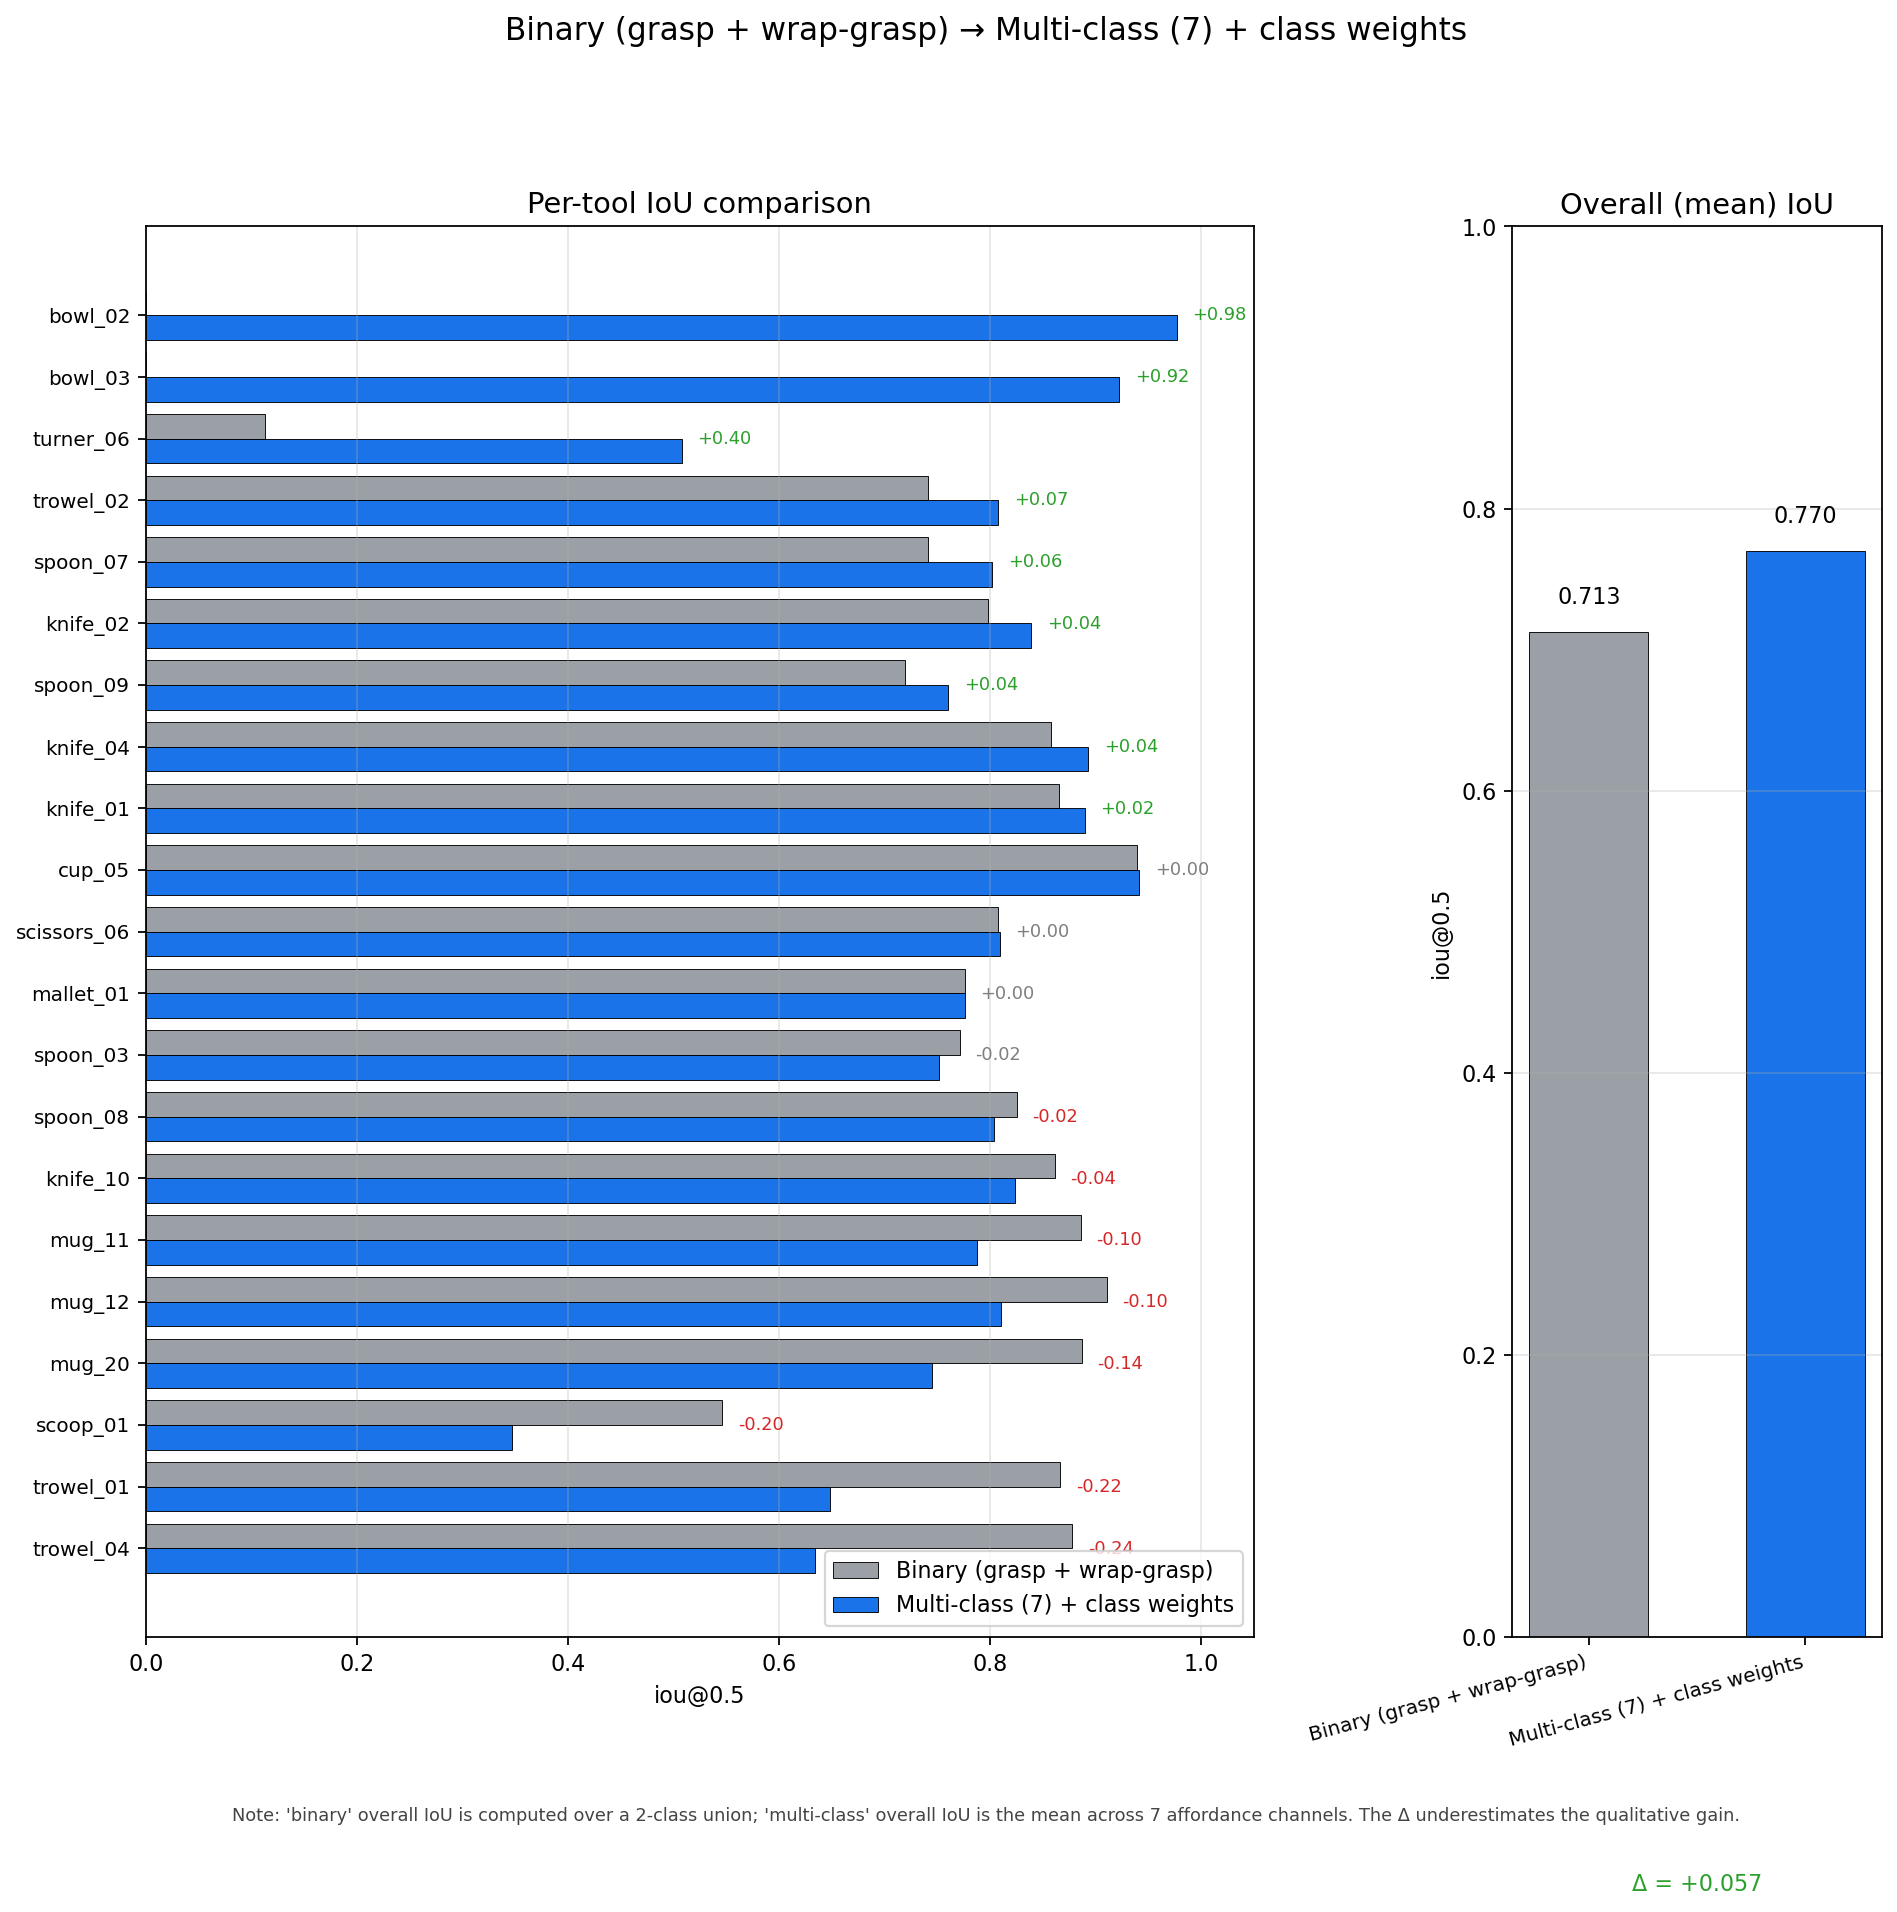
\includegraphics[width=\textwidth]{comparison_binary_vs_multiclass.png}
    \end{column}
  \end{columns}
  \medskip
  \begin{center}
    \alert{\textbf{Lesson: zero scores are diagnostics, not failures.}}
  \end{center}
\end{frame}

% =====================================================================
% 8. STORY PART 2 — RARE CLASSES
% =====================================================================
\begin{frame}{The iterative story, part 2: rare classes}
  \textbf{Phase B analysis}: rare classes overfit ---
  \texttt{support} 0.89 train / \alert{0.36 val}.
  \medskip

  \textbf{Phase C} --- frequency-inverse class weights:
  \begin{equation*}
    w_c = \left(\tfrac{N_{\text{neg}}}{N_{\text{pos}}}\right)^{0.5}
    \text{, clipped at } 15
  \end{equation*}
  \begin{itemize}
    \item \texttt{support}: $0.36 \rightarrow 0.53$ val IoU
    \item headline mean-IoU: $0.713 \rightarrow 0.770$
  \end{itemize}
  \medskip
  \textbf{Honest caveat}: heavy positive weighting buys recall at the cost of
  precision --- this returns later as the in-the-wild failure mode.
\end{frame}

% =====================================================================
% 9. THE BUG WE ALMOST SHIPPED
% =====================================================================
\begin{frame}{The bug we almost shipped}
  Augmentation rotated normal \emph{vectors} by $+\theta$ --- but in the
  y-down camera frame, the image warp corresponds to $-\theta$.
  Up to $2\theta$ ($30^\circ$!) of supervision error on every rotated sample
  --- \alert{and the training curves looked completely normal.}
  \medskip
  \begin{center}
    \begin{tabular}{lccc}
      \toprule
      mean angular error vs.\ recomputed GT & $\theta=5^\circ$ & $\theta=10^\circ$ & $\theta=15^\circ$ \\
      \midrule
      wrong sign ($+\theta$, original code) & $3.7^\circ$ & $7.5^\circ$ & $11.1^\circ$ \\
      no vector rotation at all             & $1.9^\circ$ & $3.7^\circ$ & $5.6^\circ$ \\
      \textbf{fixed} ($-\theta$)            & $\mathbf{0.2^\circ}$ & $\mathbf{0.1^\circ}$ & $\mathbf{0.2^\circ}$ \\
      \bottomrule
    \end{tabular}
  \end{center}
  \smallskip
  {\small Verified on synthetic slanted-plane depth before changing any code
  (\texttt{tests/test\_normal\_rotation.py}).}
  \medskip
  \begin{center}
    \alert{\textbf{Lesson: geometric supervision must be verified geometrically ---
    loss curves won't tell you.}}
  \end{center}
\end{frame}

% =====================================================================
% 10. FINAL RESULTS
% =====================================================================
\begin{frame}{Final results \hfill \todo{Phase D numbers}}
  \begin{columns}[T]
    \begin{column}{0.48\textwidth}
      \textbf{Headline (val, instance split)}
      \medskip
      \begin{tabular}{lcc}
        \toprule
        & Phase C & \textbf{Phase D} \\
        \midrule
        mean-IoU (per-sample)    & 0.770          & \todo{x.xxx} \\
        mean-IoU (dataset-level) & ---            & \todo{x.xxx} \\
        angular error            & $24.3^\circ$   & \todo{xx.x$^\circ$} \\
        $\leq 30^\circ$ fraction & 73.3\%         & \todo{xx\%} \\
        \bottomrule
      \end{tabular}
      \medskip
      {\small Two IoU aggregations: per-sample mean (continuity with earlier
      phases) and dataset-level (batch-size invariant, pixel-weighted ---
      the defensible headline).}
    \end{column}
    \begin{column}{0.48\textwidth}
      \todo{per-class bar chart}\par\medskip
      \todo{Phase A$\rightarrow$B$\rightarrow$C$\rightarrow$D progression
      plot --- each decision $\rightarrow$ measured delta}
    \end{column}
  \end{columns}
\end{frame}

% =====================================================================
% 11. QUALITATIVE — WHAT WORKS
% =====================================================================
\begin{frame}{What the model gets right}
  \begin{columns}[T]
    \begin{column}{0.48\textwidth}
      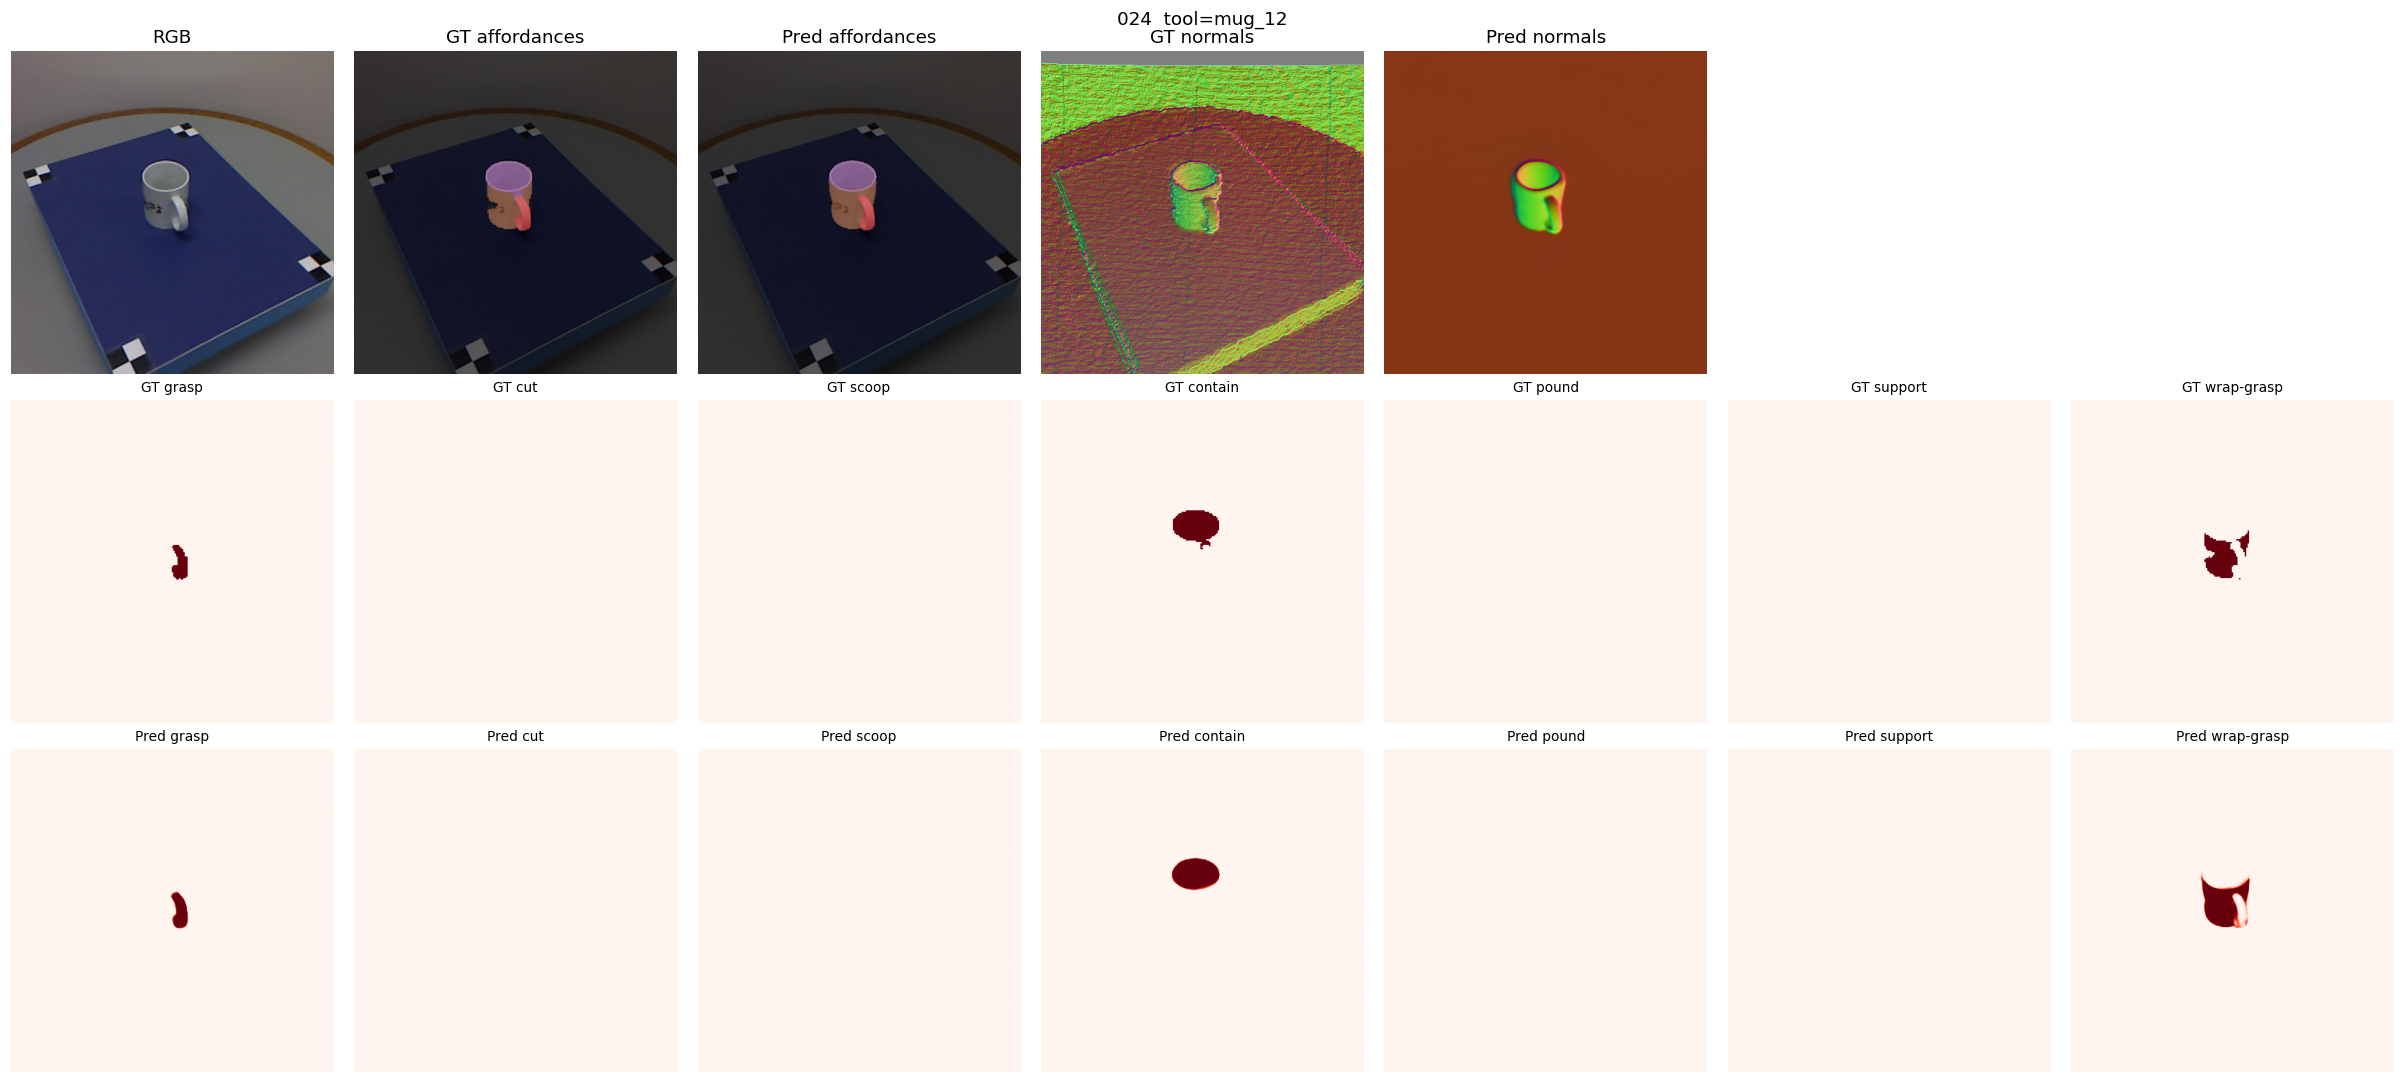
\includegraphics[width=\textwidth]{sample_mug.png}
      \par {\scriptsize Mug: three affordances simultaneously ---
      \texttt{wrap-grasp} handle, \texttt{contain} cavity, \texttt{grasp} rim.}
    \end{column}
    \begin{column}{0.48\textwidth}
      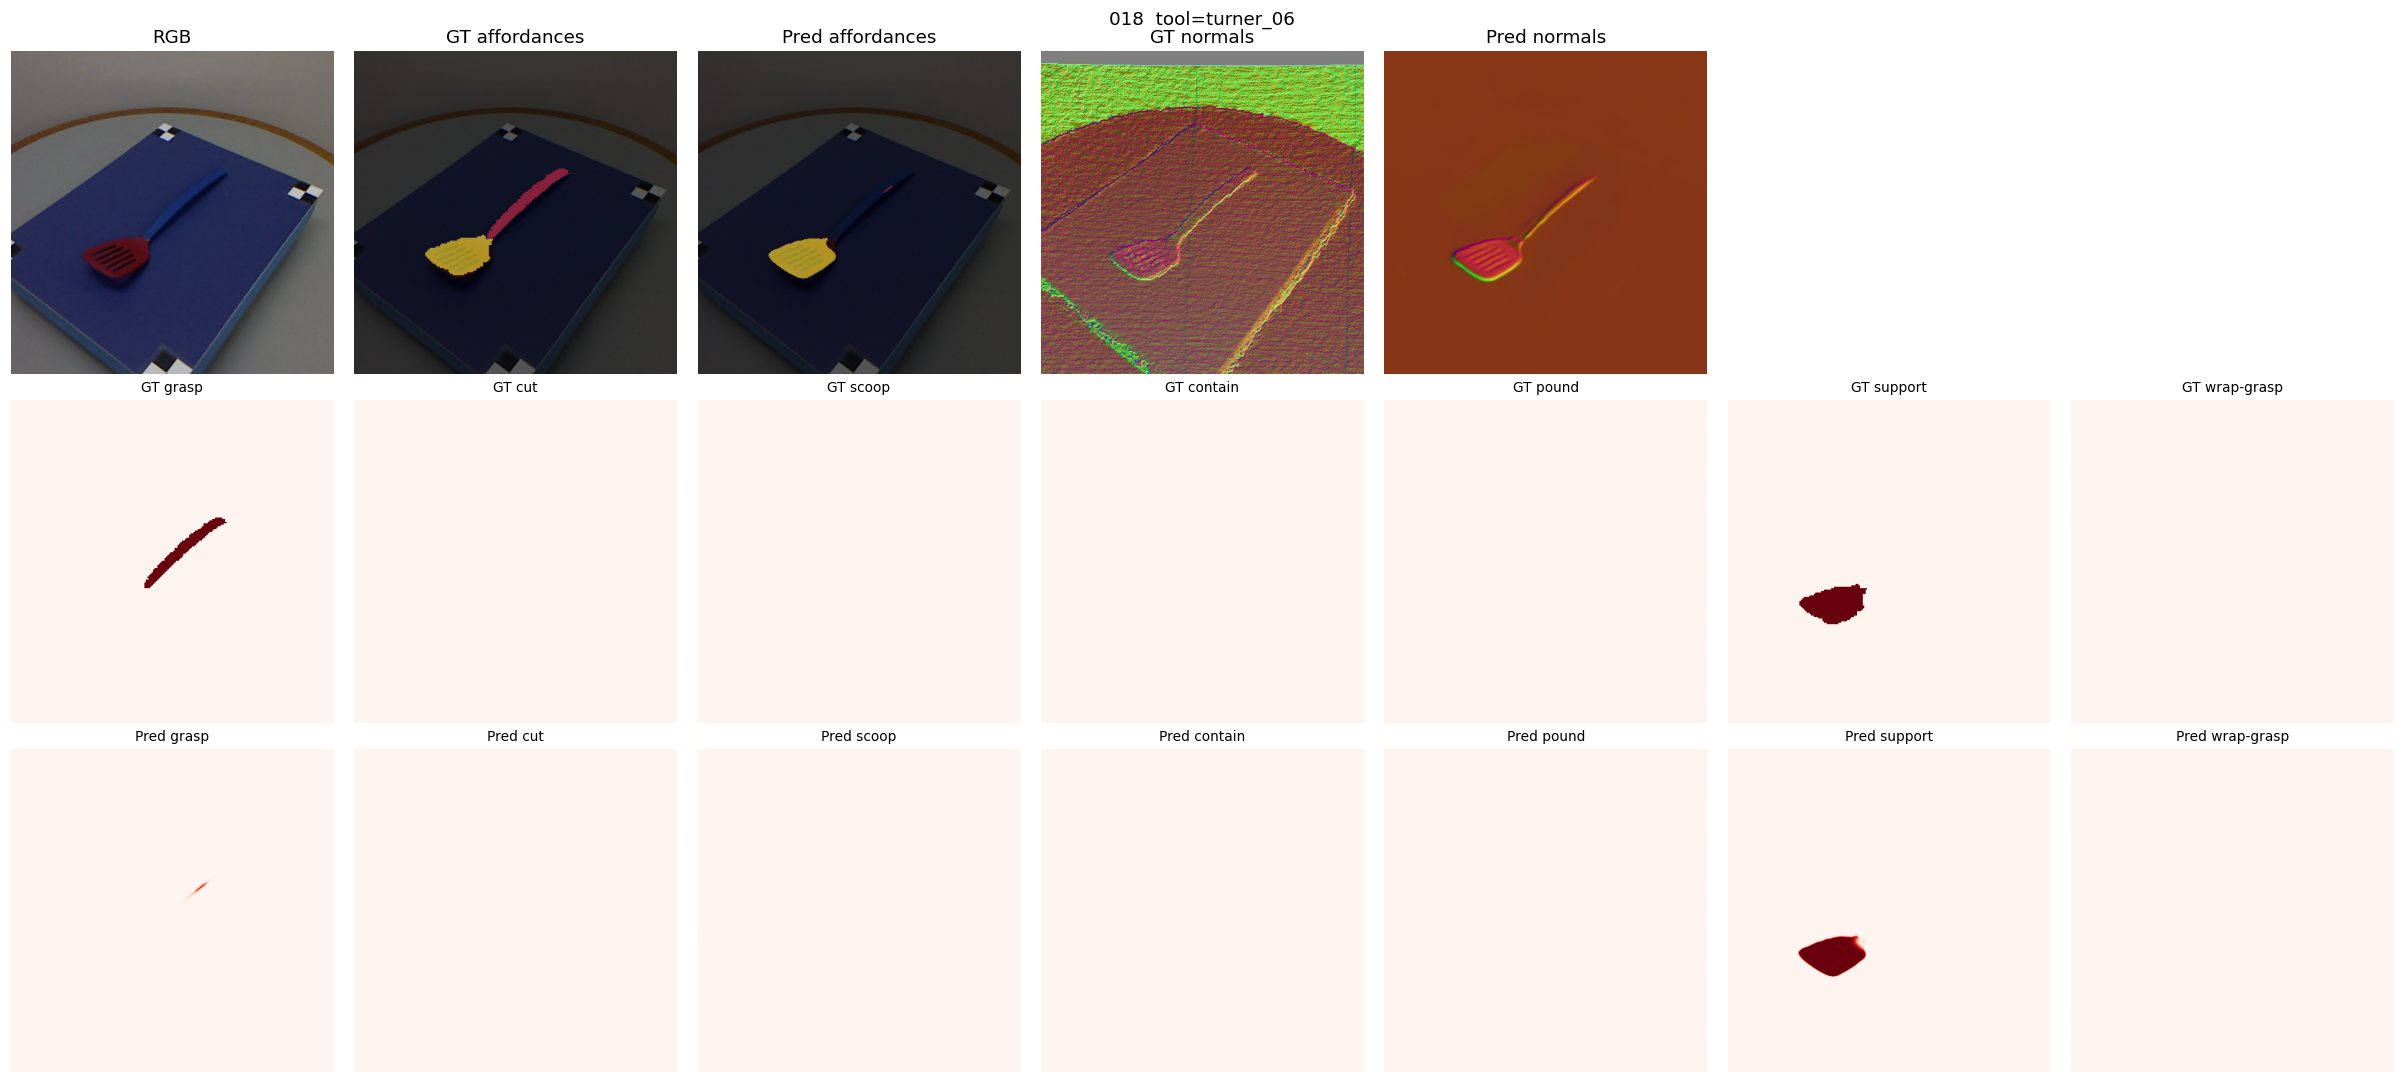
\includegraphics[width=\textwidth]{sample_turner_support.png}
      \par {\scriptsize Turner: \texttt{support} surface --- invisible to the
      binary baseline.}
    \end{column}
  \end{columns}
  \medskip
  \textbf{Observation}: predictions are often \emph{smoother than the
  hand-painted GT} --- an emergent implicit label-denoising effect.
  \hfill \todo{regenerate samples with Phase D model}
\end{frame}

% =====================================================================
% 12. IN THE WILD — WHAT BREAKS AND WHY
% =====================================================================
\begin{frame}{In the wild: what breaks, and why \hfill \todo{Phase D gallery}}
  21 phone photos, zero-shot. Transfers well \emph{within object contours} to
  novel kitchenware. Three failure modes:
  \medskip
  \begin{enumerate}
    \item \textbf{\texttt{grasp} fires on wood texture} (boards, tables) ---
          no negative supervision: ``wooden surface, not a handle'' does not
          exist in UMD.
    \item \textbf{\texttt{contain} too conservative on oblique views} ---
          turntable viewpoint bias; threshold $0.3$ recovers the area
          $\rightarrow$ calibration, not capacity.
    \item \textbf{Transparent objects fail} --- refraction and specularity
          are out of distribution.
  \end{enumerate}
  \medskip
  \begin{center}
    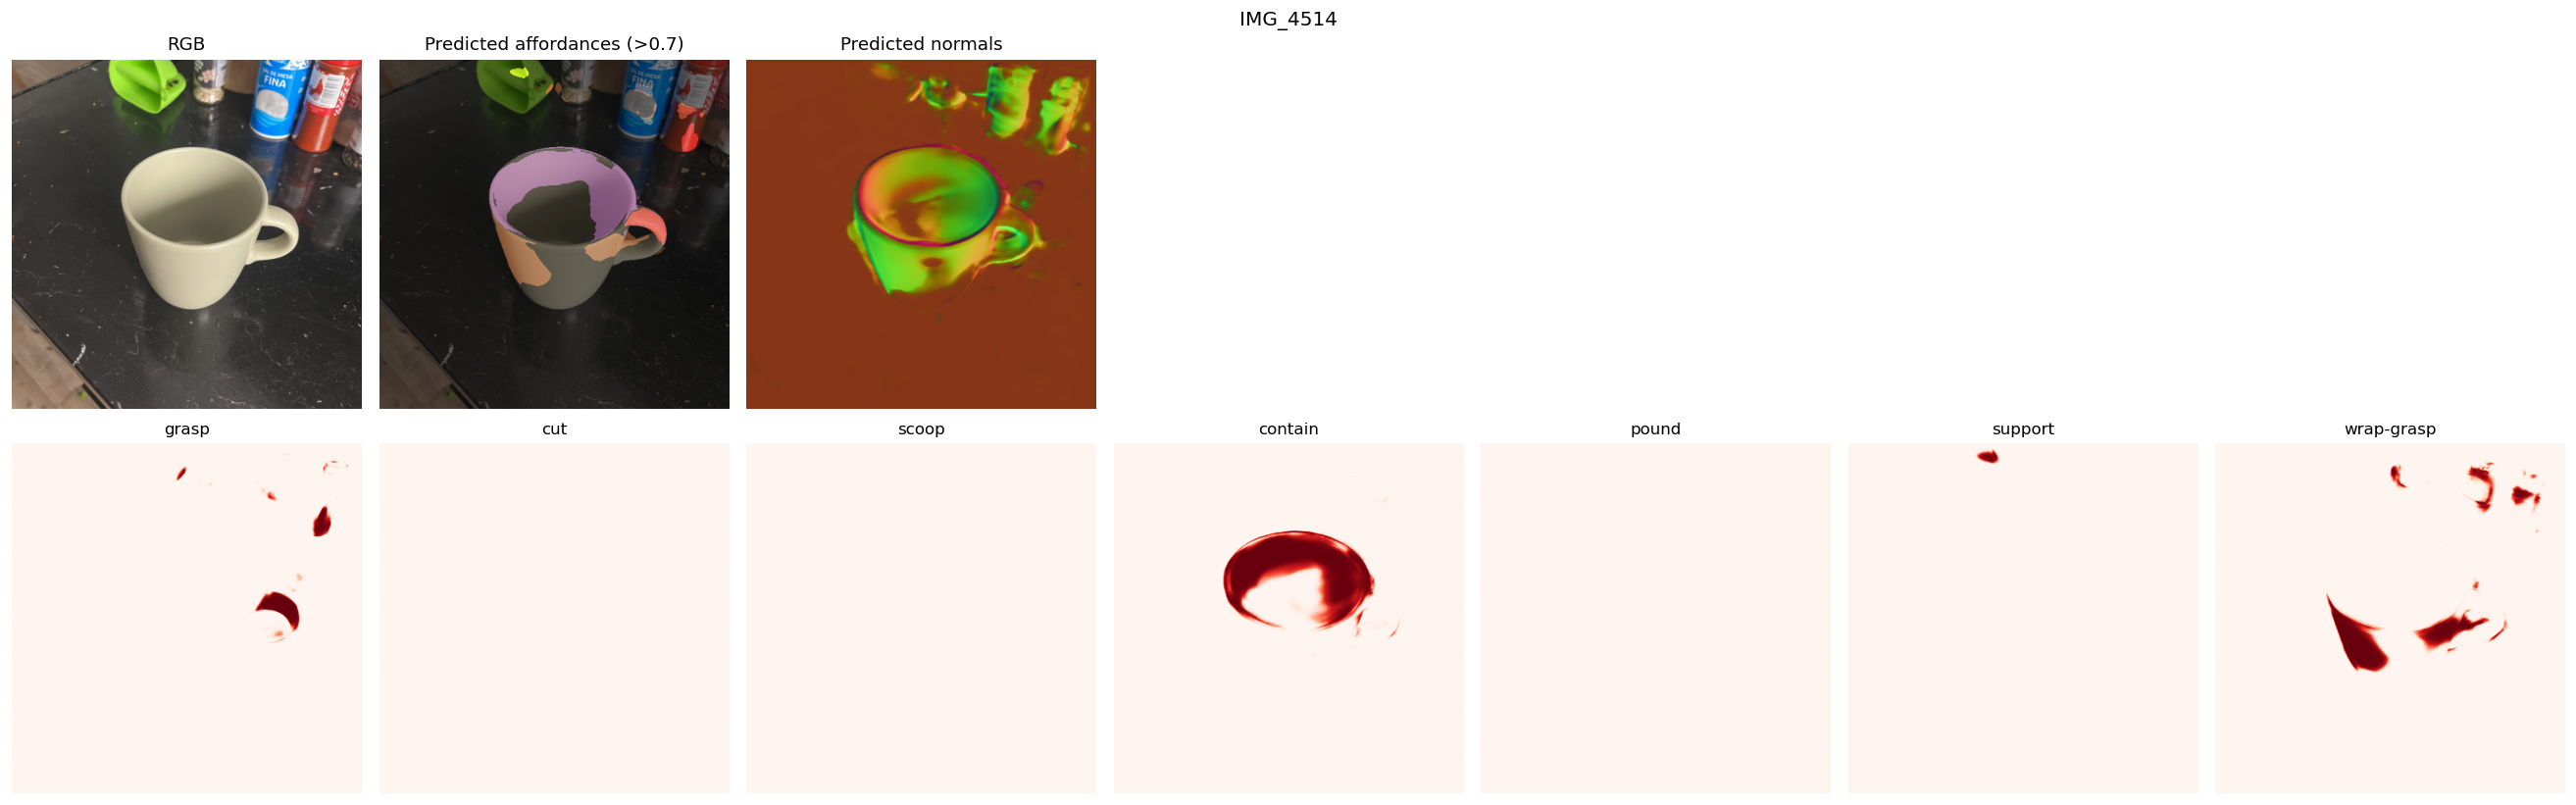
\includegraphics[height=0.30\textheight]{in_the_wild_mug.png}\hspace{1em}
    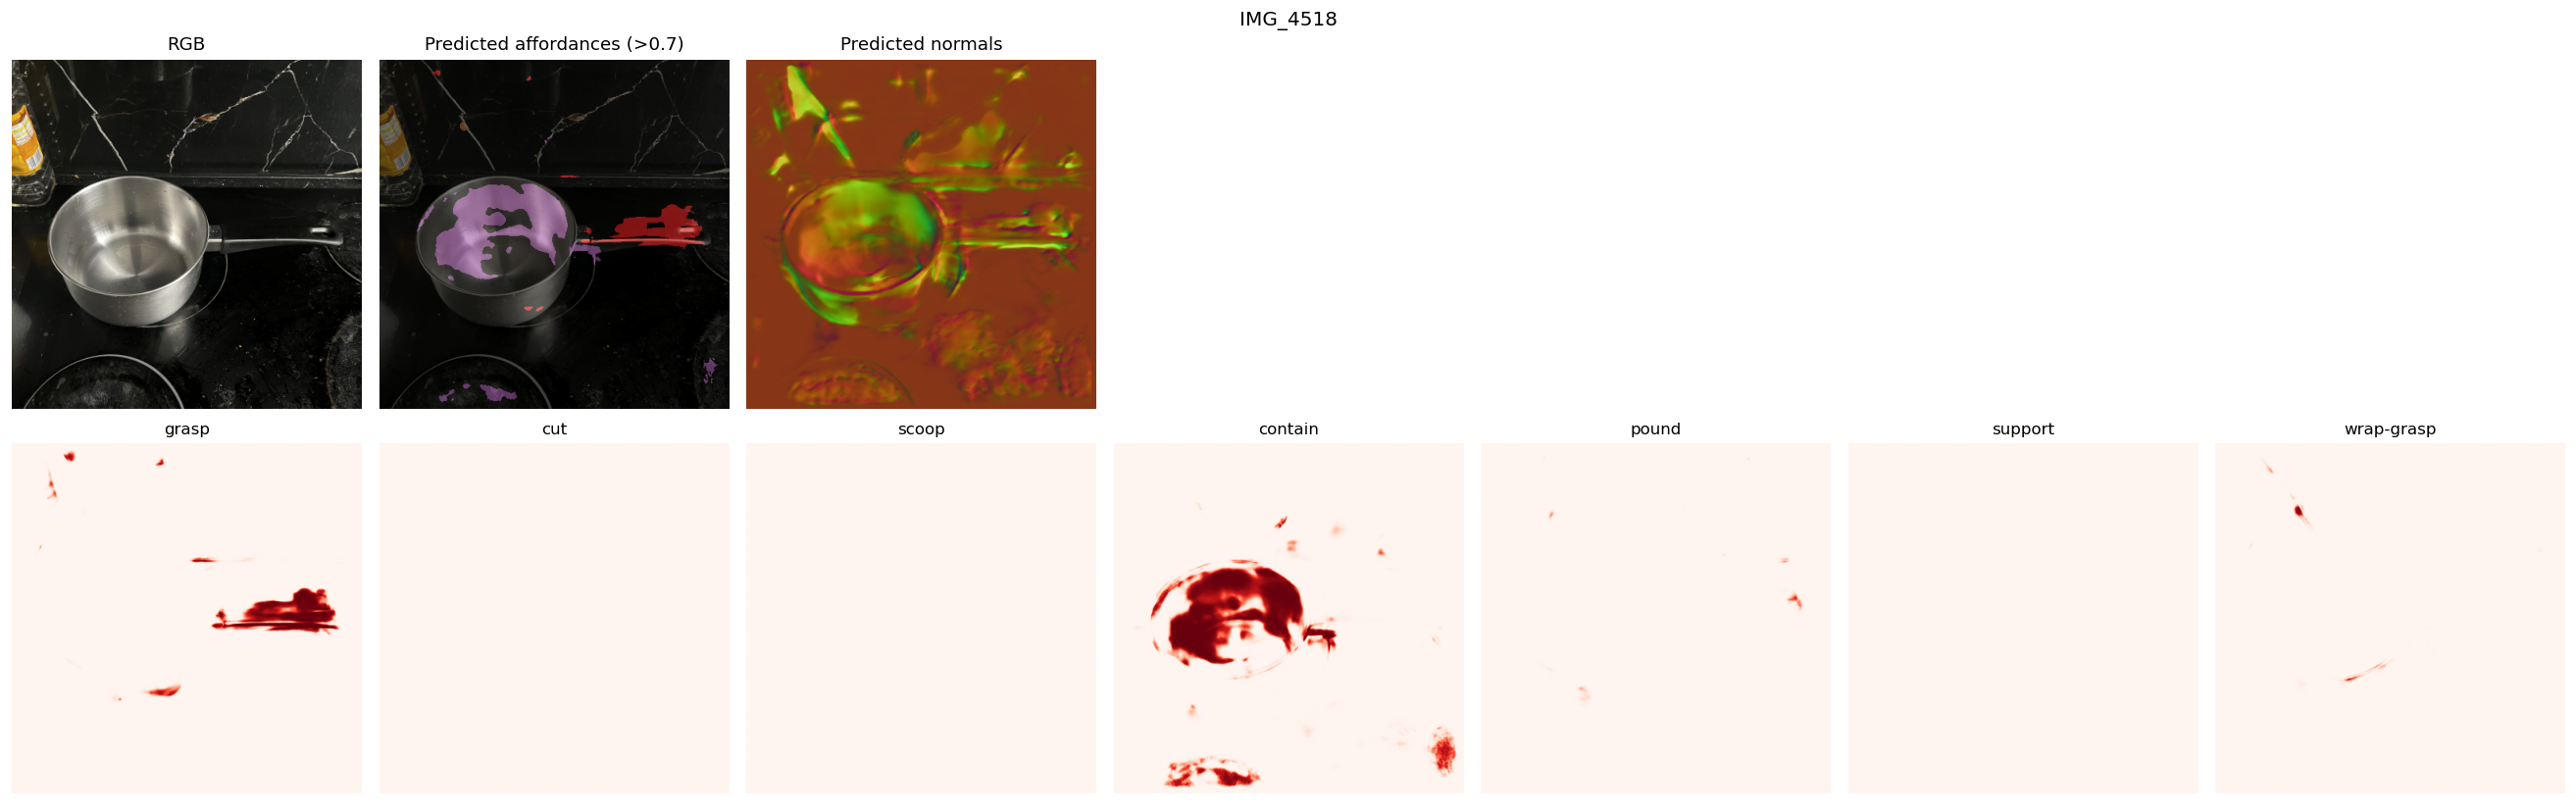
\includegraphics[height=0.30\textheight]{in_the_wild_saucepan.png}
  \end{center}
\end{frame}

% =====================================================================
% 13. LIMITATIONS & FUTURE WORK
% =====================================================================
\begin{frame}{Limitations and future work}
  \textbf{Honest limits}
  \begin{itemize}\small
    \item Single-object turntable training distribution vs.\ cluttered reality.
    \item Normals bounded by Kinect-v1 GT noise
          ($3$--$5$\,mm $\rightarrow$ $8$--$15^\circ$).
    \item Frozen-backbone capacity ceiling (val plateau confirmed).
  \end{itemize}
  \medskip
  \textbf{Roadmap (course $\rightarrow$ startup)}
  \begin{itemize}\small
    \item \alert{Factored pipeline}: SAM2 finds objects $\rightarrow$
          affordance model per crop --- directly fixes failure mode 1,
          no retraining.
    \item Text-conditioned affordance head (open vocabulary beyond 7 classes).
    \item VLA integration: perception tool today, grasp-safety verifier next.
  \end{itemize}
\end{frame}

% =====================================================================
% 14. CONCLUSIONS
% =====================================================================
\begin{frame}{Conclusions}
  \begin{enumerate}
    \item \textbf{Zero scores are diagnostics, not failures} --- the bowls'
          0.0 IoU led to the project's largest improvement.
    \item \textbf{Geometric supervision must be verified geometrically} ---
          the rotation bug was invisible in every training curve.
    \item \textbf{The metric is part of the method} --- defining the
          dataset-level IoU changed which checkpoint is ``best''.
  \end{enumerate}
  \bigskip
  \begin{center}
    Frozen DINOv2 + 3.6M-param decoder $\Rightarrow$ all 7 affordance classes
    + surface normals, RGB-only.\\
    \medskip
    \todo{final headline numbers}
  \end{center}
\end{frame}

% =====================================================================
% 15. DEMO
% =====================================================================
\begin{frame}{Demo}
  \begin{center}
    {\Large \texttt{python scripts/predict.py --input\_dir <fresh photos>}}
    \bigskip

    Live: 2--3 phone photos taken today --- 7 affordance channels + normals,
    no depth sensor, no CAD model.
    \bigskip

    {\small (Pre-rendered fallback in appendix.)}
  \end{center}
\end{frame}

\begin{frame}[standout]
  Questions?
\end{frame}

% =====================================================================
% APPENDIX — Q&A BACKUP
% =====================================================================
\appendix

\begin{frame}{Backup: why a frozen backbone?}
  28K narrow-domain images vs.\ 142M-image priors --- fine-tuning destroys
  generalisation. Partial unfreeze of the last 2--4 blocks at lr $10^{-5}$
  is the documented next step once the decoder has converged.
\end{frame}

\begin{frame}{Backup: why two IoU numbers?}
  Per-sample mean kept for continuity with Phases A--C; dataset-level
  accumulates intersection/union pixel counts over the full split and divides
  once --- invariant to batch size and sample order, weights every pixel
  equally. Checkpoint selection uses the dataset-level number.
\end{frame}

\begin{frame}{Backup: did the bug fix change mask results?}
  No --- masks carry no vector components; only the normal supervision was
  corrupted. \todo{show Phase C vs.\ D mask IoU side by side to confirm}
\end{frame}

\begin{frame}{Backup: why not train on clutter?}
  UMD clutter labels are incomplete --- the loss must ignore unlabeled regions
  rather than treat them as negatives; a project in itself. Zero-shot clutter
  evaluation is the documented next step.
\end{frame}

\begin{frame}{Backup: demo fallback}
  \todo{insert 2--3 pre-rendered prediction grids from
  \texttt{scripts/predict.py} on the same photos used in the live demo}
\end{frame}

\end{document}
